\documentclass{article}
\usepackage[utf8]{inputenc}
\usepackage{hyperref}

% graphics
\usepackage{graphicx}
\usepackage{float}
\graphicspath{{figures/}}

% todo notes
\usepackage{todonotes}
\let\oldtodo\todo
\renewcommand{\todo}[1]{\oldtodo[noline]{#1}}

% math stuff
\usepackage{amsmath}
\usepackage{amssymb}
\usepackage{amsthm}
\usepackage{commath}
\newcommand{\RR}{\mathbb{R}}
\newcommand{\NN}{\mathbb{N}}
\newcommand{\ZZ}{\mathbb{Z}}
\newcommand{\T}[1]{#1^{\top}}
\newcommand{\kth}[2][k]{#2^{(#1)}}
\newcommand{\Lip}[3]{\mathcal{F}_{#1}^{#2, #3}}
\newcommand{\Strong}[4]{\mathcal{S}_{#1, #2}^{#3, #4}}
\newcommand{\strong}[2]{\mathcal{S}_{#1}^{#2}}
\newcommand{\Lipl}{\Lip{L}{1}{1}}
\newcommand{\strongm}{\strong{\mu}{1}}
\newcommand{\Strongml}{\Strong{L}{\mu}{1}{1}}
\newcommand{\iprod}[2]{\left\langle #1, #2 \right\rangle}

\DeclareMathOperator{\diag}{diag}
\DeclareMathOperator*{\argmin}{arg min}
\DeclareMathOperator{\Span}{span}
\DeclareMathOperator{\proj}{proj}
\DeclareMathOperator{\card}{card}
\DeclareMathOperator{\tr}{tr}
\DeclareMathOperator{\rank}{rank}

\hyphenation{Lip-schitz}

% layout/sectioning
\newcounter{summary}[section]
\newcommand{\summary}[1]{%
  \paragraph{\arabic{section}.\arabic{summary}\enspace #1.}\refstepcounter{summary}}
\newcommand{\optionalsummary}[1]{%
  \paragraph{\arabic{section}.\arabic{summary}*\enspace #1.}\refstepcounter{summary}}
\renewcommand{\thesummary}{\thesection .\arabic{summary}}

\newtheoremstyle{slplain}% name
  {.5\baselineskip\@plus.2\baselineskip\@minus.2\baselineskip}% Space above
  {0pt}% Space below
  {\itshape}% Body font
  {}%Indent amount (empty = no indent, \parindent = para indent)
  {\bfseries}%  Thm head font
  {.}%       Punctuation after thm head
  { }%      Space after thm head: " " = normal interword space;
        %       \newline = linebreak
  {}%       Thm head spec
\theoremstyle{slplain}
\newtheorem{question}{Question}

\usepackage{parskip}



%%% Local Variables:
%%% mode: latex
%%% TeX-master: "summary"
%%% End:


\title{Hints for OCS Questions}
\author{Julian Wolf \and Philipp Gabler}


\begin{document}
\maketitle

\section{Basics}

%%%%%%%%%%%%%%%%%%%%%%%%%%%%%%%%%%%%%%%%%%%%%%%%%%%%%%%%%%% 
\begin{question}
  What is the definition of a general mathematical optimization problem?  Give an example and
  explain the notion of an objective function, a constraint set, an optimal solution and the
  definition of the level sets of a function.
\end{question}
Draw level lines and arrows
\begin{itemize}
\item General form:
  \begin{equation*}
    \min_{x} f(x) \quad \text{s.t. } x \in X,
  \end{equation*}
\item Objective function \(f\), constraint set \(X\).
\item A solution \(x^*\) is globally optimal if \(f(x^*) \leq f(x), \forall x \in X\) (locally, if
  this holds in an environment in \(X\) around \(x^*\)).
\item Level sets: for \(c \in \RR\), the sets
  \begin{equation*}
    S_c(f) = \{x \in X: f(x) = c\}
  \end{equation*}
  of values with equal outcome.
\end{itemize}

%%%%%%%%%%%%%%%%%%%%%%%%%%%%%%%%%%%%%%%%%%%%%%%%%%%%%%%%%%% 
\begin{question}
  Explain nonlinear programming, linear programming, quadratic programming, convex programming and
  give examples. What is the definition of a convex set and a convex function? Give examples for
  convex sets and convex functions.
\end{question}

\begin{itemize}
\item Linear: objective functions and constraints are all linear:
  \begin{equation*}
    \min_x \T{c} x, \quad\text{s.t. } Ax \leq b,\; x \geq 0.
  \end{equation*}
\item Quadratic: objective function is quadratic, constraints linear:
  \begin{equation*}
    \min_x \frac{1}{2}\T{x} Q x + \T{c} x, \quad\text{s.t. } Ax \leq b,\; Ex = d.
  \end{equation*}
  If \(Q\) is positive semidefinite, the objective is convex and the problem is polynomially
  solvable.
\item Nonlinear: no further requirements~-- objective function and constraints may be
  arbitrary.  Usually used if not known whether the problem is convex.  Not much theory available in
  general form.
\item Convex set: a set \(X\) is convex, if for all \(x, y \in X\) and
  \(\alpha \in [0,1]\):
  \begin{equation*}
    \alpha x + (1 - \alpha) y \in X.
  \end{equation*}
  This means that \(X\) contains all convex combinations of points from it.
\item Convex function: \(f: X \to \RR\) is convex if for all \(x, y \in X\) and
  \(\alpha \in [0,1]\):
  \begin{equation*}
    f(\alpha x + (1 - \alpha) y) \leq \alpha f(x) + (1 - \alpha) f(y).
  \end{equation*}
  This means that no points lie below any tangent.
\end{itemize}

%%%%%%%%%%%%%%%%%%%%%%%%%%%%%%%%%%%%%%%%%%%%%%%%%%%%%%%%%%% 
\begin{question}
  What is the difference between local and global minima. Give examples.  Give the first order
  necessary condition of optimality and prove it. What is the second order necessary condition of
  optimality? Show that for differentiable convex functions, the first order necessary condition of
  optimality becomes sufficient.
\end{question}

\begin{itemize}
\item A point \(x^*\) is called an global minimum of \(f\) if for all \(x \in X\)
  \begin{equation*}
    f(x^*) \leq f(x).
  \end{equation*}
\item \(x^*\) is called an local minimum of \(f\) if it is minimal in some neighbourhood; i.e.,
  there is an \(\epsilon > 0\) such that
  \begin{equation*}
    f(x^*) \leq f(x) \quad \forall x \text{ with } \lVert x^* - x \rVert \leq \epsilon.
  \end{equation*}
\item First order neccessary condition: If \(f\) is continuously differentiable, then in a small
  neighbourhood of \(x^*\), we can by Taylor expansion write \(f\) as
  \begin{equation*}
    f(x) = f(x^* + \Delta x) = f(x^*) + \T{\nabla f(x^*)} \Delta x + o(\lVert \Delta x \rVert).
  \end{equation*}
  Since \(x^*\) is a local minimum, \(f(x^* + \Delta x) - f(x^*) \geq 0\), and we have
  \begin{equation*}
    f(x^*) + \T{\nabla f(x^*)} \Delta x - f(x^*) = \T{\nabla f(x^*)} \Delta x \geq 0.
  \end{equation*}
  Since we can equally choose \(\Delta x\) to have the opposite sign, it holds also that
  \begin{equation*}
    \T{\nabla f(x^*)} \Delta x \leq 0,
  \end{equation*}
  so \(\T{\nabla f(x^*)} \Delta x = 0\), which, since \(\Delta x\) is arbitrary, implies that
  \(\nabla f(x^*) = 0\), which is the neccessary condition.
\item Second order neccessary condition: \(\nabla^2 f(x^*)\) must be positive semidefinite.
\item Assume \(\nabla f(x^*) = 0\), but \(x^*\) were not optimal, so there is a \(y^*\) with
  \(f(y^*) < f(x^*)\).  Then, by convexity of \(f\),
\begin{equation*}
  f(y^*) \geq f(x^*) + \iprod{\nabla f(x^*)}{y^* - x^*} = f(x^*);
\end{equation*}
this contradicts the assumption, therefore \(x^*\) must be optimal.
\end{itemize}

\begin{figure}[H]
  \centering
  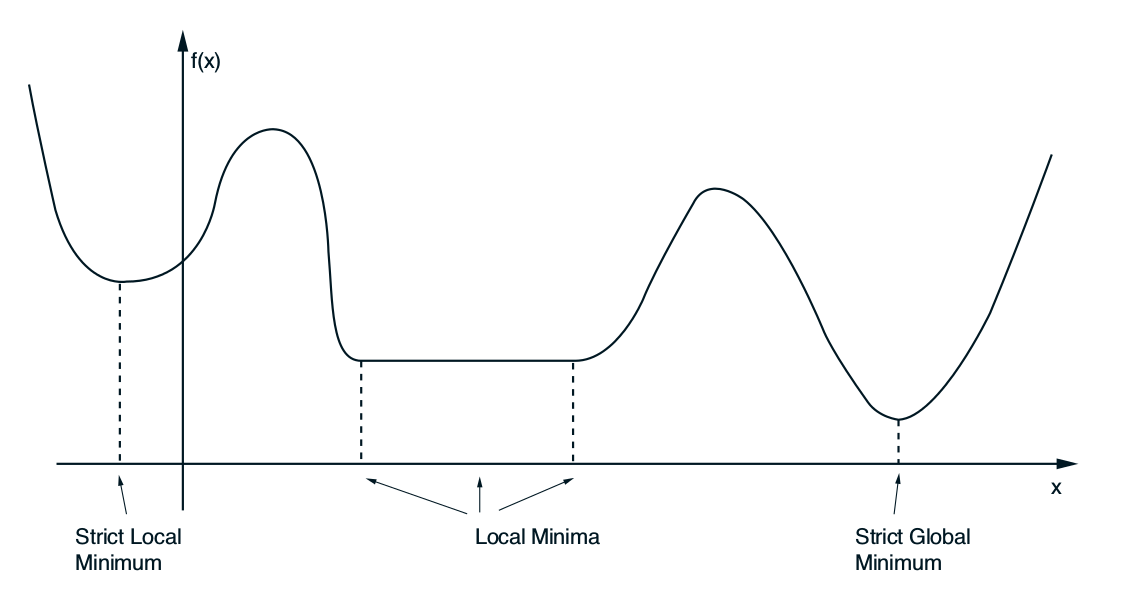
\includegraphics[width=0.8\textwidth]{loc_glob_min.png}
  \caption{Local/global minima.\label{fig:min}}
\end{figure}

%%%%%%%%%%%%%%%%%%%%%%%%%%%%%%%%%%%%%%%%%%%%%%%%%%%%%%%%%%% 
\begin{question}
  Discuss the optimality conditions for a quadratic optimization problem of the form
  \begin{equation*}
    \min_x \frac{1}{2} \T{x} Q x - \T{b} x.
  \end{equation*}
  When is this problem convex and what does convexity imply? Give a simple example in 2D showing
  different realizations of \(Q\).
\end{question}

Example for \(f: \RR \to \RR\): in this case, \(f(x) = \frac{1}{2}qx^2 + bx\). We have:
\begin{itemize}
\item First order necessessary optimality condition: \(\nabla f(x^*) = qx - b = 0\).
\item Second order necessessary optimality condition: \(\nabla^2 f(x^*) = q \geq 0\).
\end{itemize}
Since this is a parabola, we have three cases:
\begin{enumerate}
\item \(q > 0\): Unique minimum exists as minimum of upwards parabola.
\item \(q = 0\): Horizontal line, every point is locally minimal.
\item \(q < 0\): Downwards parabola, not bounded from below, so no minimum.
\end{enumerate}

Example for \(f: \RR \to \RR^2\):
\begin{itemize}
\item First order necessessary optimality condition: \(\nabla f(x^*) = Qx - b = 0\)
\item Second order necessessary optimality condition: \(\nabla^2 f(x^*) = Q\) is positive
  semidefinite.	
\end{itemize}
In more concrete form: if \(Q = \diag(\alpha, \beta)\), \(\T{b} = [1, 0]\), then
\begin{equation*}
  f(x) = \frac{1}{2} (\alpha x^2 + \beta y^2) + x.
\end{equation*}
\(Q\) is positive definite if all eigenvalues, which in this case are \(\alpha\) and \(\beta\),
are positive.  See Figure~\ref{fig:cond_quad}.  The second case is not bounded from below; the
fourth case is a saddle surface.
\begin{figure}[H]
  \centering
  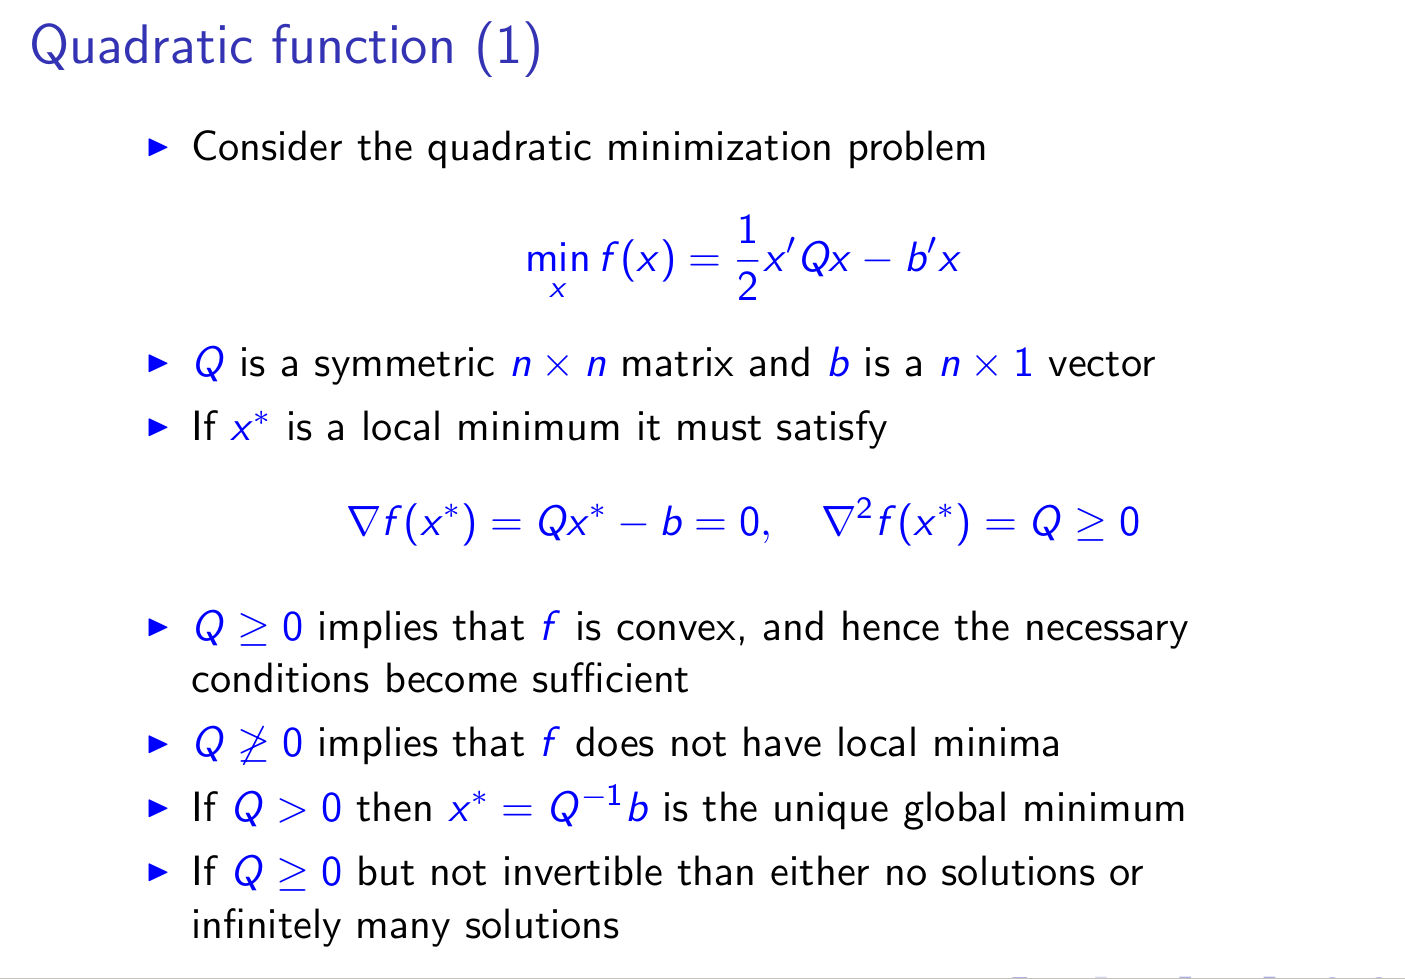
\includegraphics[width=0.6\textwidth]{cond_quad_q.png}
  \caption{Different scenarios for \(Q\).\label{fig:cond_quad}}
\end{figure}


\section{Gradient Methods, Optimality}

%%%%%%%%%%%%%%%%%%%%%%%%%%%%%%%%%%%%%%%%%%%%%%%%%%%%%%%%%%% 
\begin{question}
  What is a descent direction? Draw a simple example explaining the properties of a descent
  direction. Give the general form of a gradient method and show that
  \(\kth{d} = -\kth{D} \nabla f(x_k)\) with \(\kth{D}\) symmetric and positive definite is a descent
  direction.
\end{question}
\begin{itemize}
\item \(\kth{d}\) is a descent direction if
  \begin{equation*}
    \pd{f}{{\kth{d}}}(\kth{x}) = \T{\nabla f(\kth{x})} \kth{d} < 0
  \end{equation*}
  Interpretation: \(\kth{d}\) goes more downhill than uphill; see Figure~\ref{fig:desc_dir}.
  \begin{figure}[H]
    \centering
    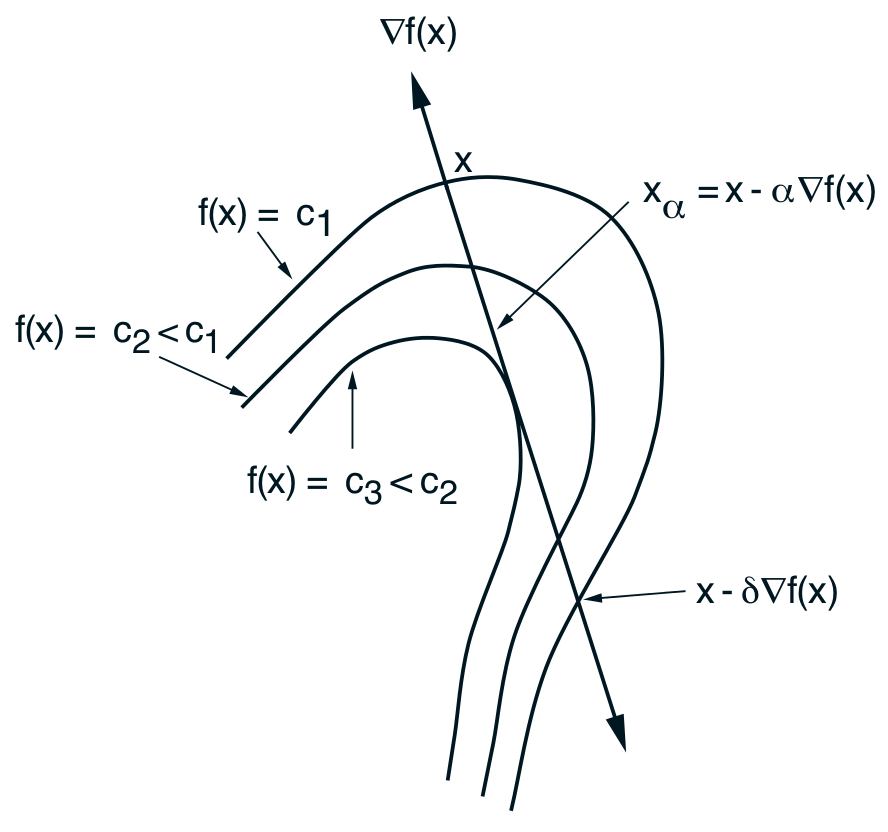
\includegraphics[width=0.5\textwidth]{desc_dir.png}
    \caption{Illustration of a descent direction.\label{fig:desc_dir}}
  \end{figure}
\item General form of gradient method:
  \begin{enumerate}
  \item Choose an initial vector \(\kth[0]{x} \in \RR^n\)
  \item Choose a descent direction \(\kth{d}\) that satisfies \(\T{\nabla f(\kth{x})} \kth{d} < 0\)
  \item Choose a positive step size \(\kth{\alpha}\)
  \item Compute the new vector as
  \begin{equation*}
    \kth[k+1]{x} = \kth{x} + \kth{\alpha} \kth{d}
  \end{equation*}
  \item Set \(k = k + 1\) and goto 2, until some termination criterion is fulfilled
\end{enumerate}
\item We have
  \begin{equation*}
    \T{\nabla f(\kth{x})} \kth{d} = -\T{\nabla f(\kth{x})} \kth{D} \nabla f(\kth{x}) < 0,
  \end{equation*}
  by direct application of the definition of positive definiteness.

\end{itemize}

%%%%%%%%%%%%%%%%%%%%%%%%%%%%%%%%%%%%%%%%%%%%%%%%%%%%%%%%%%% 
\begin{question}
  Give three different standard choices for descent directions based on choosing the scaling matrix
  \(\kth{D}\) and discuss their numerical performance. What is the Armijo step size selection
  rule? Draw an example explaining the set of acceptable step sizes.
\end{question}
Possible descent scalings:
\begin{itemize}
\item \(\kth{D} = I\): steepest descent, slow convergence if the level lines are elongated (leads to
  zig-zagging).
\item \(\kth{D} = \nabla^2 f(\kth{x})\): Newton's method, very fast convergence near minima.  Unstable in
  wrt. initial values (may diverge). Requires recalculation of inverse of Hessian in every step~--
  very expensive in large dimensions.
\item \(\kth{d} = \del[1]{\pd[2]{f(\kth{x})}{(x_i)}}^2\): diagonal scaling, an approximation of
  Newton's method, but usually not worth it (scales only in diagonal directions).
\item \(\kth{d} = \del[1]{\nabla g(\kth{x}) \T{\nabla g(\kth{x})}}^{-1}\): Gauss-Newton method, for
  least squares problems with design function \(g\). Good performance; again calculation of inverse,
  but not of the Hessian.
\end{itemize}

Armijo rule: it is not sufficient to simply ensure that \(f(\kth[k+1]{x}) < f(\kth{x})\). To apply
it, we fix scalars \(s\), \(0 < \beta < 1\), and \(0 < \sigma < 1\), and set
\(\kth{\alpha} = \beta^{m_k} s\), where we choose \(m_k\) as the first nonnegative integer for which
\begin{equation*}
  f(\kth{x} + \beta^{m_k} s \kth{d}) - f(\kth{x}) \leq \sigma \beta^{m_k} s \nabla \T{f(\kth{x})} \kth{d}.
\end{equation*}
Thus, the step sizes are chosen such that the energy decrease is sufficiently large~-- see
Figure~\ref{fig:armijo}.
\begin{figure}[H]
  \centering
  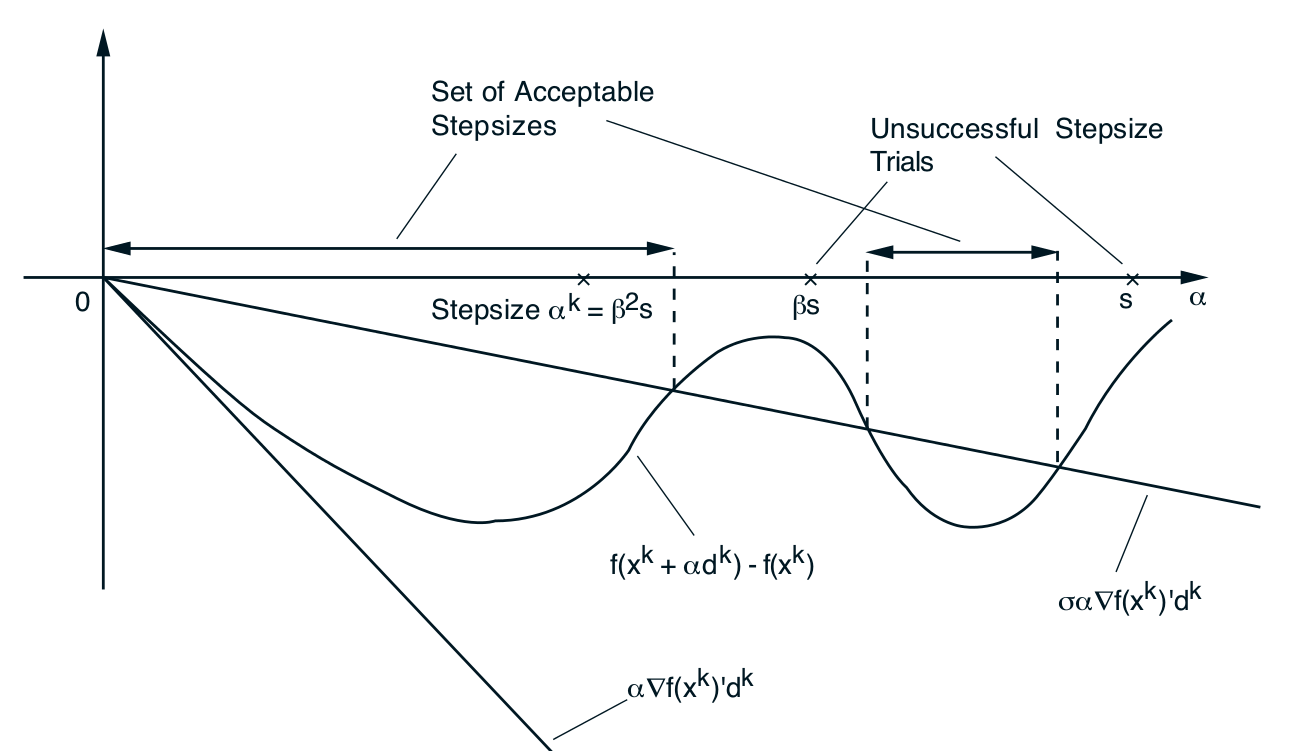
\includegraphics[width=0.8\textwidth]{armijo.png}
  \caption{Graphical representation of the idea of the Armijo rule.\label{fig:armijo}}
\end{figure}


\section{Convergence}

%%%%%%%%%%%%%%%%%%%%%%%%%%%%%%%%%%%%%%%%%%%%%%%%%%%%%%%%%%% 
\begin{question}
  What is a Lipschitz continuous gradient, and what is the descent lemma?  Give the proof of the
  descent lemma.
\end{question}

A differentiable function \(f: \RR^n \to \RR\) has Lipschitz continuous gradient if there is
a Lipschitz constant \(L \geq 0\), such that for all \(x, y \in \RR^n\)
\begin{equation*}
  \enVert{\nabla f(x) - \nabla f(y)} \leq L \enVert[1]{x - y},
\end{equation*}
or equivalently
\begin{equation*}
  \enVert{\nabla f(x + ty) - \nabla f(x)} \leq Lt \enVert[1]{y} \quad \forall t \in [0, 1]
\end{equation*}
for some norm.

Let \(f: \RR^n \to \RR\) have an \(L\)-Lipschitz continuous gradient.  Then for all \(x, y\), we
have the following quadratic upper bound on the objective function at \(x\):
\begin{equation*}
  f(y) \leq f(x) + \iprod{\nabla f(x)}{y - x} + \frac{L}{2}\enVert{y - x}^2,
\end{equation*}
Proof: let \(g(t) = f(x + t(y - x))\), so that \(g(0) = f(x)\) and \(g(1) = f(y)\). Then
\begin{align*}
  f(y) &= f(x) + f(y) - f(x) \\
       &= f(x) + g(1) - g(0) \\
       &= f(x) + \int_0^1 g'(t) \dif t \\
       &= f(x) + \int_0^1 \T{\nabla f(x + t(y - x))} (y - x) \dif t \\
       &= f(x) + \int_0^1 \iprod{\nabla f(x)}{y - x} \dif t
         + \int_0^1 \iprod{\nabla f(x + t(y - x)) - \nabla f(x)}{y - x} \dif t \\
       &\overset{(1)}{\leq} f(x) + \iprod{\nabla f(x)}{y - x}
         + \int_0^1 \enVert[1]{\nabla f(x + t(y - x)) - \nabla f(x)}\! \cdot \enVert[1]{y - x} \dif t \\
       &\overset{(2)}{\leq} f(x) + \iprod{\nabla f(x)}{y - x} + \enVert[1]{y - x} \int_0^1 Lt\enVert[1]{y - x} \dif t \\
       &= f(x) + \iprod{\nabla f(x)}{y - x} + \frac{L}{2}\enVert[1]{y - x}^2,
\end{align*}
where (1) is an application of the Cauchy-Schwarz theorem
(\(\langle x, y \rangle \leq \enVert{x} \cdot \enVert{y}\)), and (2) follows from Lipschitz
continuity of the gradient

%%%%%%%%%%%%%%%%%%%%%%%%%%%%%%%%%%%%%%%%%%%%%%%%%%%%%%%%%%% 
\begin{question}
  What is a rate of convergence? Explain linear, superlinear, and sublinear convergence and give
  examples.
\end{question}

We measure convergence in terms of asymtotic rates of a step-dependent error function
\(e: \RR^n \to \RR\) with \(e(x^*) = 0\).  The usual choices are
\begin{gather*}
  e(x) = \enVert[1]{x - x^*}, \text{ or } \\
  e(x) = f(x) - f(x^*)
\end{gather*}

Classes of convergence rates (see Figure~\ref{fig:convergence}):
\begin{enumerate}
\item Sublinear: \(\limsup_{k \to \infty} \frac{e(\kth[k+1]{x})}{e(\kth{x})} = 1\). Example:
  \(e(\kth{x}) \sim 1/(k + 1)^2\) (black curve; this does not imply that the method does not
  converge!).
\item Linear: \(\limsup_{k \to \infty} \frac{e(\kth[k+1]{x})}{e(\kth{x})} \leq \beta \in (0, 1)\).
  Example: \(e(\kth{x}) \sim 1/2^k\) (blue curve)
\item Superlinear: \(\limsup_{k \to \infty} \frac{e(\kth[k+1]{x})}{e(\kth{x})} = 0\). Example:
  \(e(\kth{x}) \sim 1/2^{2^k}\) (red curve).
\end{enumerate}

\begin{figure}[H]
  \centering
  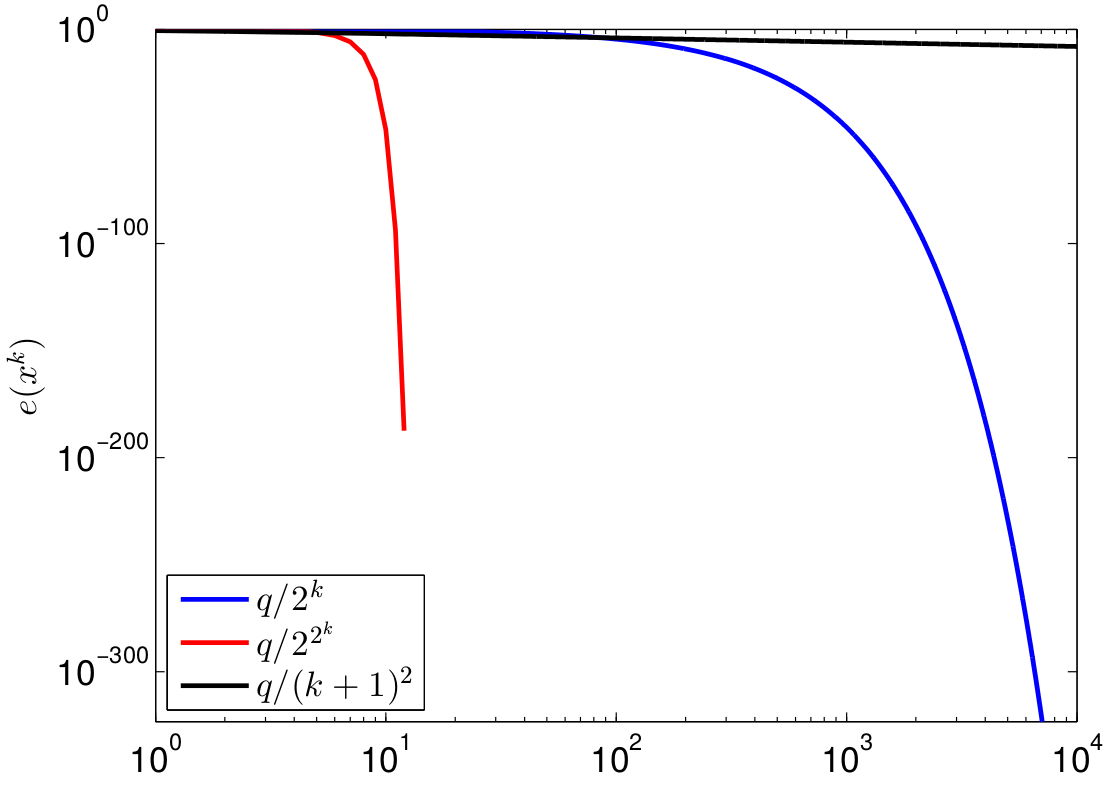
\includegraphics[width=0.7\textwidth]{convergence.png}
  \caption{Graphical representation of linear, superinear and sublinear
    convergence \label{fig:convergence}}
\end{figure}

\section{Newton's method}

%%%%%%%%%%%%%%%%%%%%%%%%%%%%%%%%%%%%%%%%%%%%%%%%%%%%%%%%%%% 
\begin{question}
  Show that the plain form of Newton’s method can be derived from a second order Taylor
  approximation of the objective function. Show that Newton’s method is invariant with respect to an
  affine change of the coordinate system.
\end{question}

Newton's method is base on the sequence
\begin{equation*}
  \kth[k+1]{x} = \kth{x} - \kth{\alpha}\left( \nabla^2 f(\kth{x}) \right)^{-1} \nabla f(\kth{x}).
\end{equation*}

By Taylor approximation, given a point \(\kth{x}\), we can approximate a function
\(f \in \mathcal{C}^2\) locally as
\begin{equation*}
  \kth{f}(x) = f(\kth{x}) + \T{\nabla f(\kth{x})}(x - \kth{x})
  + \frac{1}{2} \T{(x - \kth{x})} \nabla^2 f(\kth{x})(x - \kth{x}).
\end{equation*}
We can analytically minimize this approximation, which gives the stated update rule:
\begin{align*}
  \nabla \kth{f}(x) = \nabla f(\kth{x}) + \nabla^2 f(\kth{x})(x - \kth{x}) &\overset{!}{=} 0 \\
  \nabla^2 f(\kth{x})(x - \kth{x}) &= -\nabla f(\kth{x}) \\
  (x - \kth{x}) &= -(\nabla^2 f(\kth{x}))^{-1} \nabla f(\kth{x}) \\
  x = \kth[k+1]{x} &= \kth{x} - (\nabla^2 f(\kth{x}))^{-1} \nabla f(\kth{x}).
\end{align*}

Scale invariance: if we exchange \(x = Sy\) for a nonsingular \(S\), the generated steps will remain
the same.  First, observe that
\begin{align*}
  \nabla_y f(Sy) &= \T{S} \nabla f(Sy), \\
  \nabla_y^2 f(Sy) &= \T{S} \nabla^2 f(Sy) S.
\end{align*}
Now, the second-order approximation around \(S\kth{y}\) becomes
\begin{align*}
  \kth{f}(Sy) &= f(S\kth{y}) + \T{(\T{S} \nabla f(Sy))}(y - \kth{y}) \\
  &\qquad + \frac{1}{2} \T{(y - \kth{y})} \nabla^2 f(S\kth{y}) (y - \kth{y}),
\end{align*}
which we can minimize at \(\kth[k+1]{y}\) to get the update rule, like above:
\begin{align*}
  & &\nabla \kth{f}(\kth[k+1]{y}) &= \T{S} \nabla f(S\kth{y}) + \T{S} \nabla^2
                                 f(S\kth{y})S(\kth[k+1]{y}
                                 - \kth{y}) \overset{!}{=} 0 \\
  &\Rightarrow & S\kth[k+1]{y} &= S\kth{y} - \left( \T{S}\nabla^2 f(S\kth{y}) \right)^{-1} \T{S}
                                  \nabla f(S\kth{y}) \\
  &\phantom{\Rightarrow} & &= S\kth{y} - \nabla^2 f(S\kth{y})^{-1} (\T{S})^{-1}
                                 \T{S} \nabla f(S\kth{y}) \\
  &\Rightarrow & S\kth[k+1]{y} &= S\kth{y} - \nabla^2 f(S\kth{y})^{-1} \nabla f(S\kth{y}) \\
  &\Leftrightarrow & \kth[k+1]{x} &= \kth{x} - \nabla^2 f(\kth{x})^{-1} \nabla f(\kth{x}).
\end{align*}

\section{Least squares problems}

%%%%%%%%%%%%%%%%%%%%%%%%%%%%%%%%%%%%%%%%%%%%%%%%%%%%%%%%%%% 
\begin{question}
  What are linear (and nonlinear) least squares problems?  Give an example.  What is the Gauss-Newton
  method, and what is its relation to Newton’s method?
\end{question}

We want to minimize
\begin{equation*}
  f(x) = \frac{1}{2} \enVert[1]{g(x)}^2 = \frac{1}{2} \sum_i \enVert[1]{g_i(x)}^2,
\end{equation*}
for a continuously differentiable function \(g\) with components \(g_i\), which can be linear or
nonlinear.  This is equivalent to solving the problem \(g(x) = 0\), a possibly overdetermined
system.

Often, a least squares problem is a model fitting problem, where
\begin{equation*}
  g_i(\theta) = h(x_i, \theta) - \hat{y}_i
\end{equation*}
is the loss for a single sample for a model function \(h\) with parameters \(\theta\), samples
\(x_i\), and targets~\(\hat{y}_i\).  If we take, e.g., a linear predictor, we would have the form
\(g_i(\theta) = \T{\theta} x_i - \hat{y}_i\), which we can put together in matrix form as
\(g(\theta) = Ax - y\) with the so-called model matrix \(A\).

To derive the Gauss-Newton method, we replace \(g\) by a local approximation around \(\kth{x}\):
\begin{equation*}
  \tilde{g}(x, \kth{x}) = g(\kth{x}) + \T{\nabla g(\kth{x})}(x - \kth{x}).
\end{equation*}
This leads to a step method of the form
\begin{equation*}
  \kth[k+1]{x} = \kth{x} - \left(\nabla g(\kth{x}) \T{\nabla g(\kth{x})}\right)^{-1} \T{\nabla g(\kth{x})} g(\kth{x}),
\end{equation*}
assuming that \((\nabla g(\kth{x}) \T{\nabla g(\kth{x})}\) is invertible.

To compare with Newton's method, look at the derivatives
\begin{align*}
  \nabla f(x) &= \T{\nabla g(x)} g(x), \\
  \nabla^2 f(x) &= \nabla g(x) \T{\nabla g(x)} + \sum_i \nabla^2 g_i(x) g_i(x).
\end{align*}
Neglecting the second-order part in the Hessian, this reduces to a form equivalent to Newton's
method, but saving the computation of the full Hessian (intuitively,
\(\nabla^2 g \approx (\nabla g)^2\)).


%%%%%%%%%%%%%%%%%%%%%%%%%%%%%%%%%%%%%%%%%%%%%%%%%%%%%%%%%%% 
\begin{question}
  What is a Kalman filter? How does it relate to an optimization problem?  What is an extended
  Kalman filter?
\end{question}

If a least-squares model (ie. the functions \(g_i\)) is linear, one Gauss-Newton iteration would be
enough to find the optimal solution (this amounts to the analytical solution using the Moore-Penrose
pseudoinverse).  However, we can develop an incremental method for this, avoiding the matrix
inversion, and instead using one sample at a time.

Concretely, for \(g_i(x) = z_i - C_i x_i\), we have a step method
\begin{align*}
  \xi_i &= \xi_{i-1} + H_i^{-1}\T{C_i}(z_i - C_i \xi_{i-1}), \quad\text{with} \\
  H_i &= \lambda H_{i-1} + \T{C_i}C_i, \\
  H_0 &= 0,\quad \xi_0 \text{ arbitrary}.
\end{align*}
(here \(H_i\) and \(C_i\) are relatively small, compared to \(\nabla g(\kth{x})\).)

If the \(g_i\) are nonlinear, we can use a linearization at the last available iteration
\(\xi_{i-1}\) to get the extended Kalman filter.  The iteration scheme stays the same, but the model
parts must be adapted to
\begin{align*}
  \tilde{z}_i &= g_i(\xi_{i-1}) + \T{\nabla g_i(\xi_{i-1})}(z_i - \xi_{i-1}), \\
  C_i &= - \T{\nabla g_i(\xi_{i-1})}.
\end{align*}

\section{Accelerated gradient methods}

%%%%%%%%%%%%%%%%%%%%%%%%%%%%%%%%%%%%%%%%%%%%%%%%%%%%%%%%%%% 
\begin{question}
  What is the lower bound of first order methods on quadratic problems?  What is an optimal
  algorithm for quadratic problems?
\end{question}

A quadratic minimization problem
\begin{equation*}
  \min_x f(x) = \frac{1}{2} \T{x} Q x - \T{b}x,
\end{equation*}
is automatically convex for positive semidefinite \(Q\).  The lower bounds for first-order gradient
methods then depend only on the eigenvalues of \(Q\), since they fix \(L = \lambda_{\text{max}}\)
and \(\mu = \lambda_{\text{min}}\): if \(Q \succeq 0\) (just positive semidefinite), then
\begin{equation*}
  f(\kth{x}) - f(x^*) \geq \frac{3\lambda_{\text{max}} \enVert[1]{\kth[0]{x} - x^*}}{32(k+1)^2}.
\end{equation*}
If \(Q \succ 0\) (positive definite, therefore a strongly convex problem), then
\begin{equation*}
  \enVert[1]{\kth{x} - x^*}
  \geq \left( \frac{\sqrt{\lambda_{\text{max}}/\lambda_{\text{min}}} - 1}{
      \sqrt{\lambda_{\text{max}}/\lambda_{\text{min}}} + 1} \right)^k \enVert[1]{\kth[0]{x} - x^*}.
\end{equation*}  
An optimal first order method for these cases is the conjugate gradient method.

%%%%%%%%%%%%%%%%%%%%%%%%%%%%%%%%%%%%%%%%%%%%%%%%%%%%%%%%%%% 
\begin{question}
  Write down the conjugate gradient (CG) method and specialize the algorithm for solving a
  least-squares problem of the form
  \[
    \min_x f(x) = \frac{1}{2} \T{x} Q x - \T{b} x.
  \]
  What is the relation to solving linear system of equations?
\end{question}

The steps in the CG method for a quadratic problem have the form
\begin{equation*}
  \kth[k+1]{x} = \kth{x} + \kth{\alpha}\kth{d},
\end{equation*}
where
\begin{equation*}
  \kth{d} = -\kth{g} + \kth{\beta}\kth[k-1]{d},
\end{equation*}
and \(\kth{\beta}\) is given by
\begin{equation*}
  \kth{\beta} = \frac{\T{(\kth{g})}\kth{g}}{\T{(\kth[k-1]{g})}\kth[k-1]{g}}.
\end{equation*}

For this concrete problem, we set
\begin{equation*}
  \kth{g} = \nabla f(\kth{x}) = Q \kth{x} - b,
\end{equation*}
and calculate the descent directions as
\begin{align*}
  \kth[0]{d} &= -\kth[0]{g}, \\
  \kth[k]{d} &= -\kth{g} + \kth{\beta}\kth[k-1]{d},
\end{align*}
where \(\kth{\beta}\) is given by
\begin{equation*}
  \kth{\beta} = \frac{\T{(\kth{g})}\kth{g}}{\T{(\kth[k-1]{g})}\kth[k-1]{g}}.
\end{equation*}

When solving a linear system \(Ax = y\), we are essentially also looking for an \(x\) which
minimizes the expression \(\enVert{Ax - y}\).  This is a special form of a quadratic problem, which
we can solve using CG.

%%%%%%%%%%%%%%%%%%%%%%%%%%%%%%%%%%%%%%%%%%%%%%%%%%%%%%%%%%%
\begin{question}
  Explain the difference between the heavy-ball algorithm and Nesterov’s algorithm.  What are the
  rates of convergence of those algorithms on strongly convex problems?
\end{question}
\begin{itemize}
\item Heavy-ball: idea is like in physics: a ball uses its momentum it gained beforehand to overcome
  small increases or flat areas of its way:
  \begin{equation*}
    \kth[k+1]{x} = \kth{x} - \kth{\alpha} \nabla f(\kth{x}) + \kth{\beta}(\kth{x} - \kth[k-1]{x}).
  \end{equation*}
\item Nesterov: instead of calculating the gradient at the current point, use a gradient step based
  on the point extrapolated from the momentum:
  \begin{align*}
    \kth{y} &= \kth{x} + \kth{\beta}(\kth{x} - \kth[k-1]{x}), \\
    \kth[k+1]{x} &= \kth{y} - \alpha\nabla f(\kth{y}).
  \end{align*}
\item Both algorithms are optimal for strongly convex functions, with
    \begin{equation*}
    f(\kth{x}) - f(x^*) \leq (1 - \sqrt{L/\mu})^k
    \left( f(\kth[0]{x}) - f(x^*) + \frac{\mu}{2} \enVert[1]{x^* - \kth[0]{x}}^2 \right)
  \end{equation*}
  for Nesterov's method and
  \begin{equation*}
    \enVert[1]{\kth{x} - x^*}^2 \leq
    \left( \frac{\sqrt{L/\mu} - 1}{\sqrt{L/\mu} + 1} \right)^{2k} \enVert[1]{\kth[0]{x} - x^*}^2.
  \end{equation*}
  for the heavy-ball method (for optimal choices of parameters).  Note that while the latter rate
  appears to be better, they are asymptotically of the same order.
\item However, only Nesterov's method is optimal for non-strong problems, since the step size
  parameters cannot be chosen correctly in the other case (since \(\mu = 0\)).  It overcomes this
  difficulty by a dynamic choice of \(\kth{\beta}\), leading to a still optimal rate of
  \begin{equation*}
    f(\kth{x}) - f(x^*) \leq \frac{2L\enVert[1]{\kth[0]{x} - x^*}^2}{(k + 1)^2}.
  \end{equation*}
\end{itemize}

\section{Constrained optimization}

%%%%%%%%%%%%%%%%%%%%%%%%%%%%%%%%%%%%%%%%%%%%%%%%%%%%%%%%%%%
\begin{question}
  Give an example showing the necessary optimality condition for minimizing a differentiable
  function over a convex set. Why does it fail in case the feasible set is non-convex?
\end{question}

The neccessary condition for optimality for a convex constraint set \(X\) is
\begin{equation*}
  \T{\nabla f(x^*)}(x - x^*) \geq 0, \quad\forall x \in X;
\end{equation*}
ie., the gradient in all feasible directions must be less than \(0\). 

For illustration, see Figure~\ref{fig:non-convex}: if a local minimum is at the boundary of \(X\) (which
will be the most interesting case, otherwise the problem is not much different from an unconstrained
one), we only need to consider directions (other points) inside the boundary, which for a convex set
implies that the gradient makes an an angle of \(90^\circ\) or less with the feasible directions.
In the non-convex case, this condition can fail.

\begin{figure}[H]
  \centering
  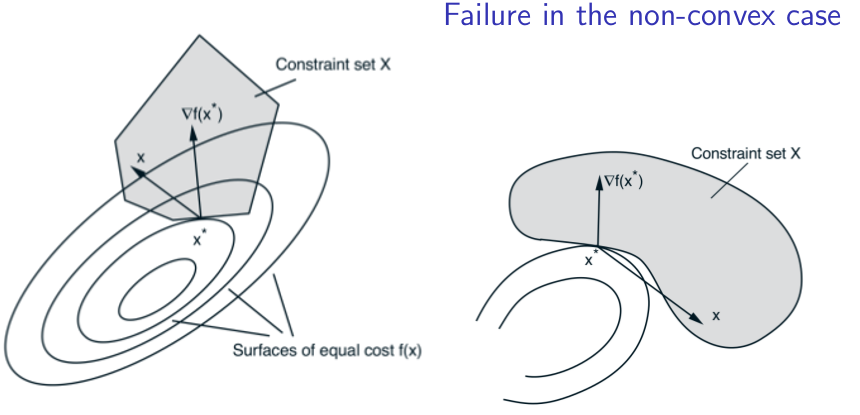
\includegraphics[width=0.8\textwidth]{non_convex.png}
  \caption{Graphical representation of convex and non-convex set \label{fig:non-convex}}
\end{figure}

%%%%%%%%%%%%%%%%%%%%%%%%%%%%%%%%%%%%%%%%%%%%%%%%%%%%%%%%%%%
\begin{question}
  What is a projection on a convex set? Give the optimality condition and specialize the condition
  to the case where the convex set is a subspace.  What are the properties of a subspace?
\end{question}

Let \(z \in \RR^n\).  The projection of \(z\) onto X is defined by
\begin{equation*}
  \proj_X(z) = \min_{x \in X}\, \frac{1}{2}\enVert[1]{x - z}^2 \quad\text{s.t. } x \in X
\end{equation*}
It is the point in \(X\) which is closest to \(z\). 

Since \(f(x) = \frac{1}{2} \enVert{x - z}^2\), we have \(\nabla f(x) = x - z\).  By the (neccessary
and sufficient) optimality condition we get that
\begin{alignat*}{2}
  &\quad & \T{\nabla f(x^*)}(x - x^*) &\geq 0 \\
  &\Leftrightarrow\quad & \T{(x - z)}(x - x^*) &\geq 0 \\
  &\Leftrightarrow\quad & \T{(z - x)}(x - x^*) &\leq 0.
\end{alignat*}
If \(X\) is a linear subspace of \(\RR^n\), this reduces to
\begin{equation*}
  \T{(z - x^*)}x = 0, \quad\forall x \in X,
\end{equation*}
since for all \(x \in X\), both \(x^* + x\) and \(x^* - x\) are in \(X\).

A linear subspace \(Y \subseteq X\) is a subset of \(X\) which is also a vector space, i.e., it is
an abelian group with respect to addition and behaves as expected with scalar multiplication.  In
particular, it contains the zero vector.

%%%%%%%%%%%%%%%%%%%%%%%%%%%%%%%%%%%%%%%%%%%%%%%%%%%%%%%%%%%
\begin{question}
  What is a feasible direction? Give an example. What is the general form of a feasible direction
  method? Also give an alternative form of the feasible direction based on a feasible vector
  \(\bar{x}\).
\end{question}
middle/end of pages slide 10 - start in interior and just take small steps $->$ we can ignore
constraint under these conditions
\begin{itemize}
\item Given a feasible vector $x$, a feasible
  direction at $x$ is a vector $d$ such that the
  vector $x + \alpha d$ is feasible for all sufficiently
  small $\alpha > 0$.
\item a feasable method generates starts at $x^0$ and generates multiple such points $x^{k+1}$
\end{itemize}

%%%%%%%%%%%%%%%%%%%%%%%%%%%%%%%%%%%%%%%%%%%%%%%%%%%%%%%%%%%
\begin{question}
  Explain the conditional gradient method and the projected gradient method.  What is different? For
  both methods draw a simple example showing how the feasible directions are computed.
\end{question}
\begin{itemize}
\item Conditional gradient solves subproblem with linear cost, gradient projection method solves
  quadratic cost fct
\item The conditional gradient method generates the point $\overline{x}^k$ by finding a feasible
  point which is furthest way from $x^k$ along the negative gradient direction $-\nabla f (x^k )$.

\end{itemize}
\begin{figure}[H]
  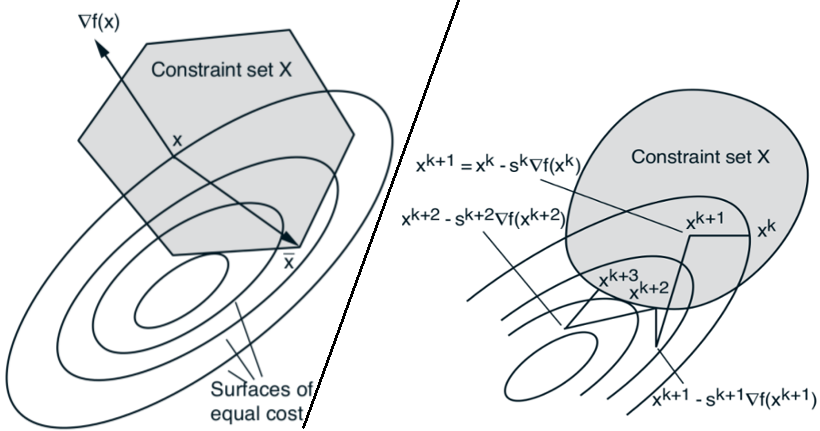
\includegraphics[width=\textwidth]{proj_desc.png}
  \caption{Graphical representation of conditional (left) and projective (right)
    method\label{fig:proj_desc}}
\end{figure}

%%%%%%%%%%%%%%%%%%%%%%%%%%%%%%%%%%%%%%%%%%%%%%%%%%%%%%%%%%%
\begin{question}
  What is the affine scaling method for solving an equality constrained LP? Show how the LP is
  solved based on solving a sequence of linearly constrained quadratic programs. Why can the
  inequality constraint be skipped?
\end{question}
\begin{itemize}
\item iterative method $x^{k+1} = x^k + \alpha^k (H^k)^{-1} (\texttt{big AHA formula})$
\item affine scaling: choose $H^k = (X^k)^{-2}$, $X^k = diag(x_1, ..., x_n)$ leads to
  $y^{k+1} = y^k + \alpha^k (AX^k A' )^{-1} b $, $\alpha^k$ ensures $x^{k+1} > 0$
\end{itemize}

%%%%%%%%%%%%%%%%%%%%%%%%%%%%%%%%%%%%%%%%%%%%%%%%%%%%%%%%%%%
\begin{question}
  What is the Lagrange multiplier theorem for equality constrained optimization problems? Draw a
  simple example and explain why the gradients of the constraint functions need to be linearly
  independent.
\end{question}
\begin{itemize}
\item Interpretation 1: The gradient of the cost function $\nabla f (x^*)$
  belongs to the subspace spanned by the gradients of the
  constraint functions $\nabla h_i (x^* )$
\item Interpretation 2: The cost gradient $\nabla f (x^* )$ is orthogonal to
  the subspace of first order feasible directions
\item for failure see figure~\ref{fig:ex1}. The Eigenvectors are lineary dependent, we loose one
  dimension and thus we can not optimize the problem (at least I think so)
\end{itemize}

%%%%%%%%%%%%%%%%%%%%%%%%%%%%%%%%%%%%%%%%%%%%%%%%%%%%%%%%%%%
\begin{question}
  Show how to solve the projection problem:
  \[
    \min_x \frac{1}{2} \enVert{x - y}^2
  \]
  Write down the Lagrangian, give the KKT conditions and show how the
problem is solved.
\end{question}

%%%%%%%%%%%%%%%%%%%%%%%%%%%%%%%%%%%%%%%%%%%%%%%%%%%%%%%%%%% 
\begin{question}
  Show how to compute the projection onto a half space:
  \[
    \min_x \frac{1}{2} \enVert{x-y}^2 \quad \text{s.t.} \quad \T{a}x = b
  \]
  Write down the Lagrangian, give the KKT conditions and show how the
  problem is solved.
\end{question}


\begin{figure}[H]
  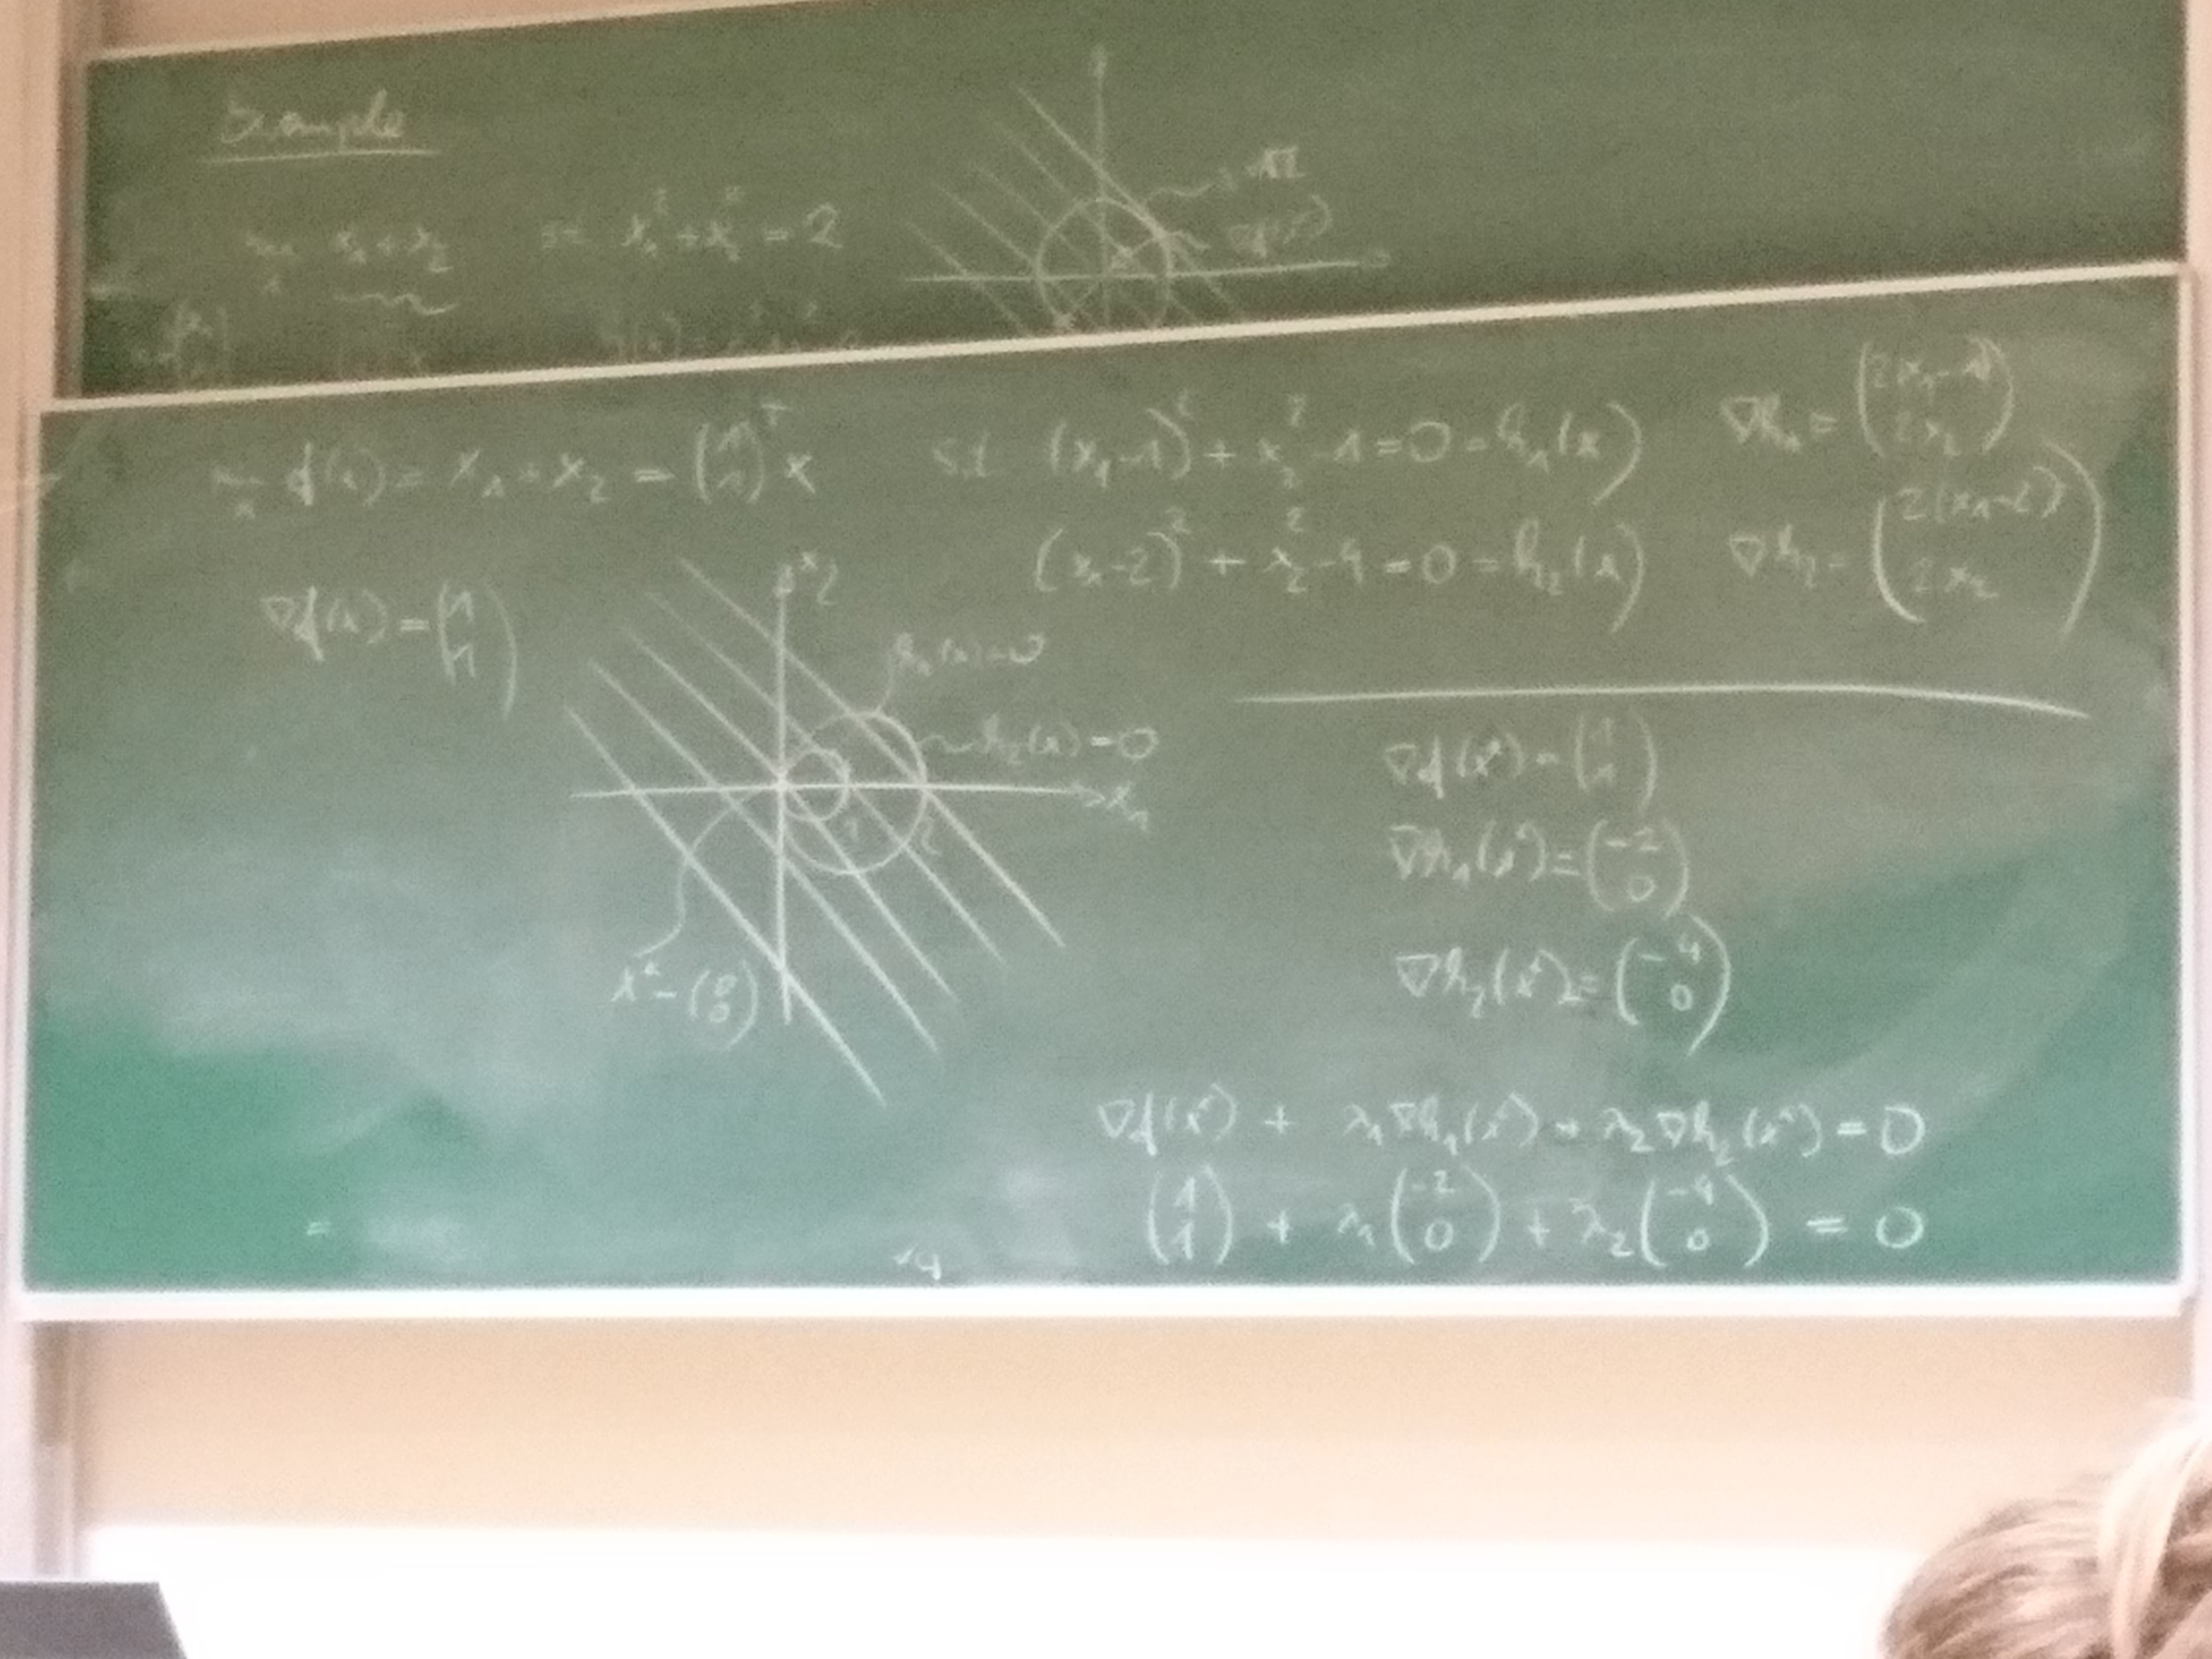
\includegraphics[width=\textwidth]{2017_01_24-ex1.jpg}
  \caption{Example1,  24.01.2017\label{fig:ex1}}
\end{figure}

\begin{figure}[H]
  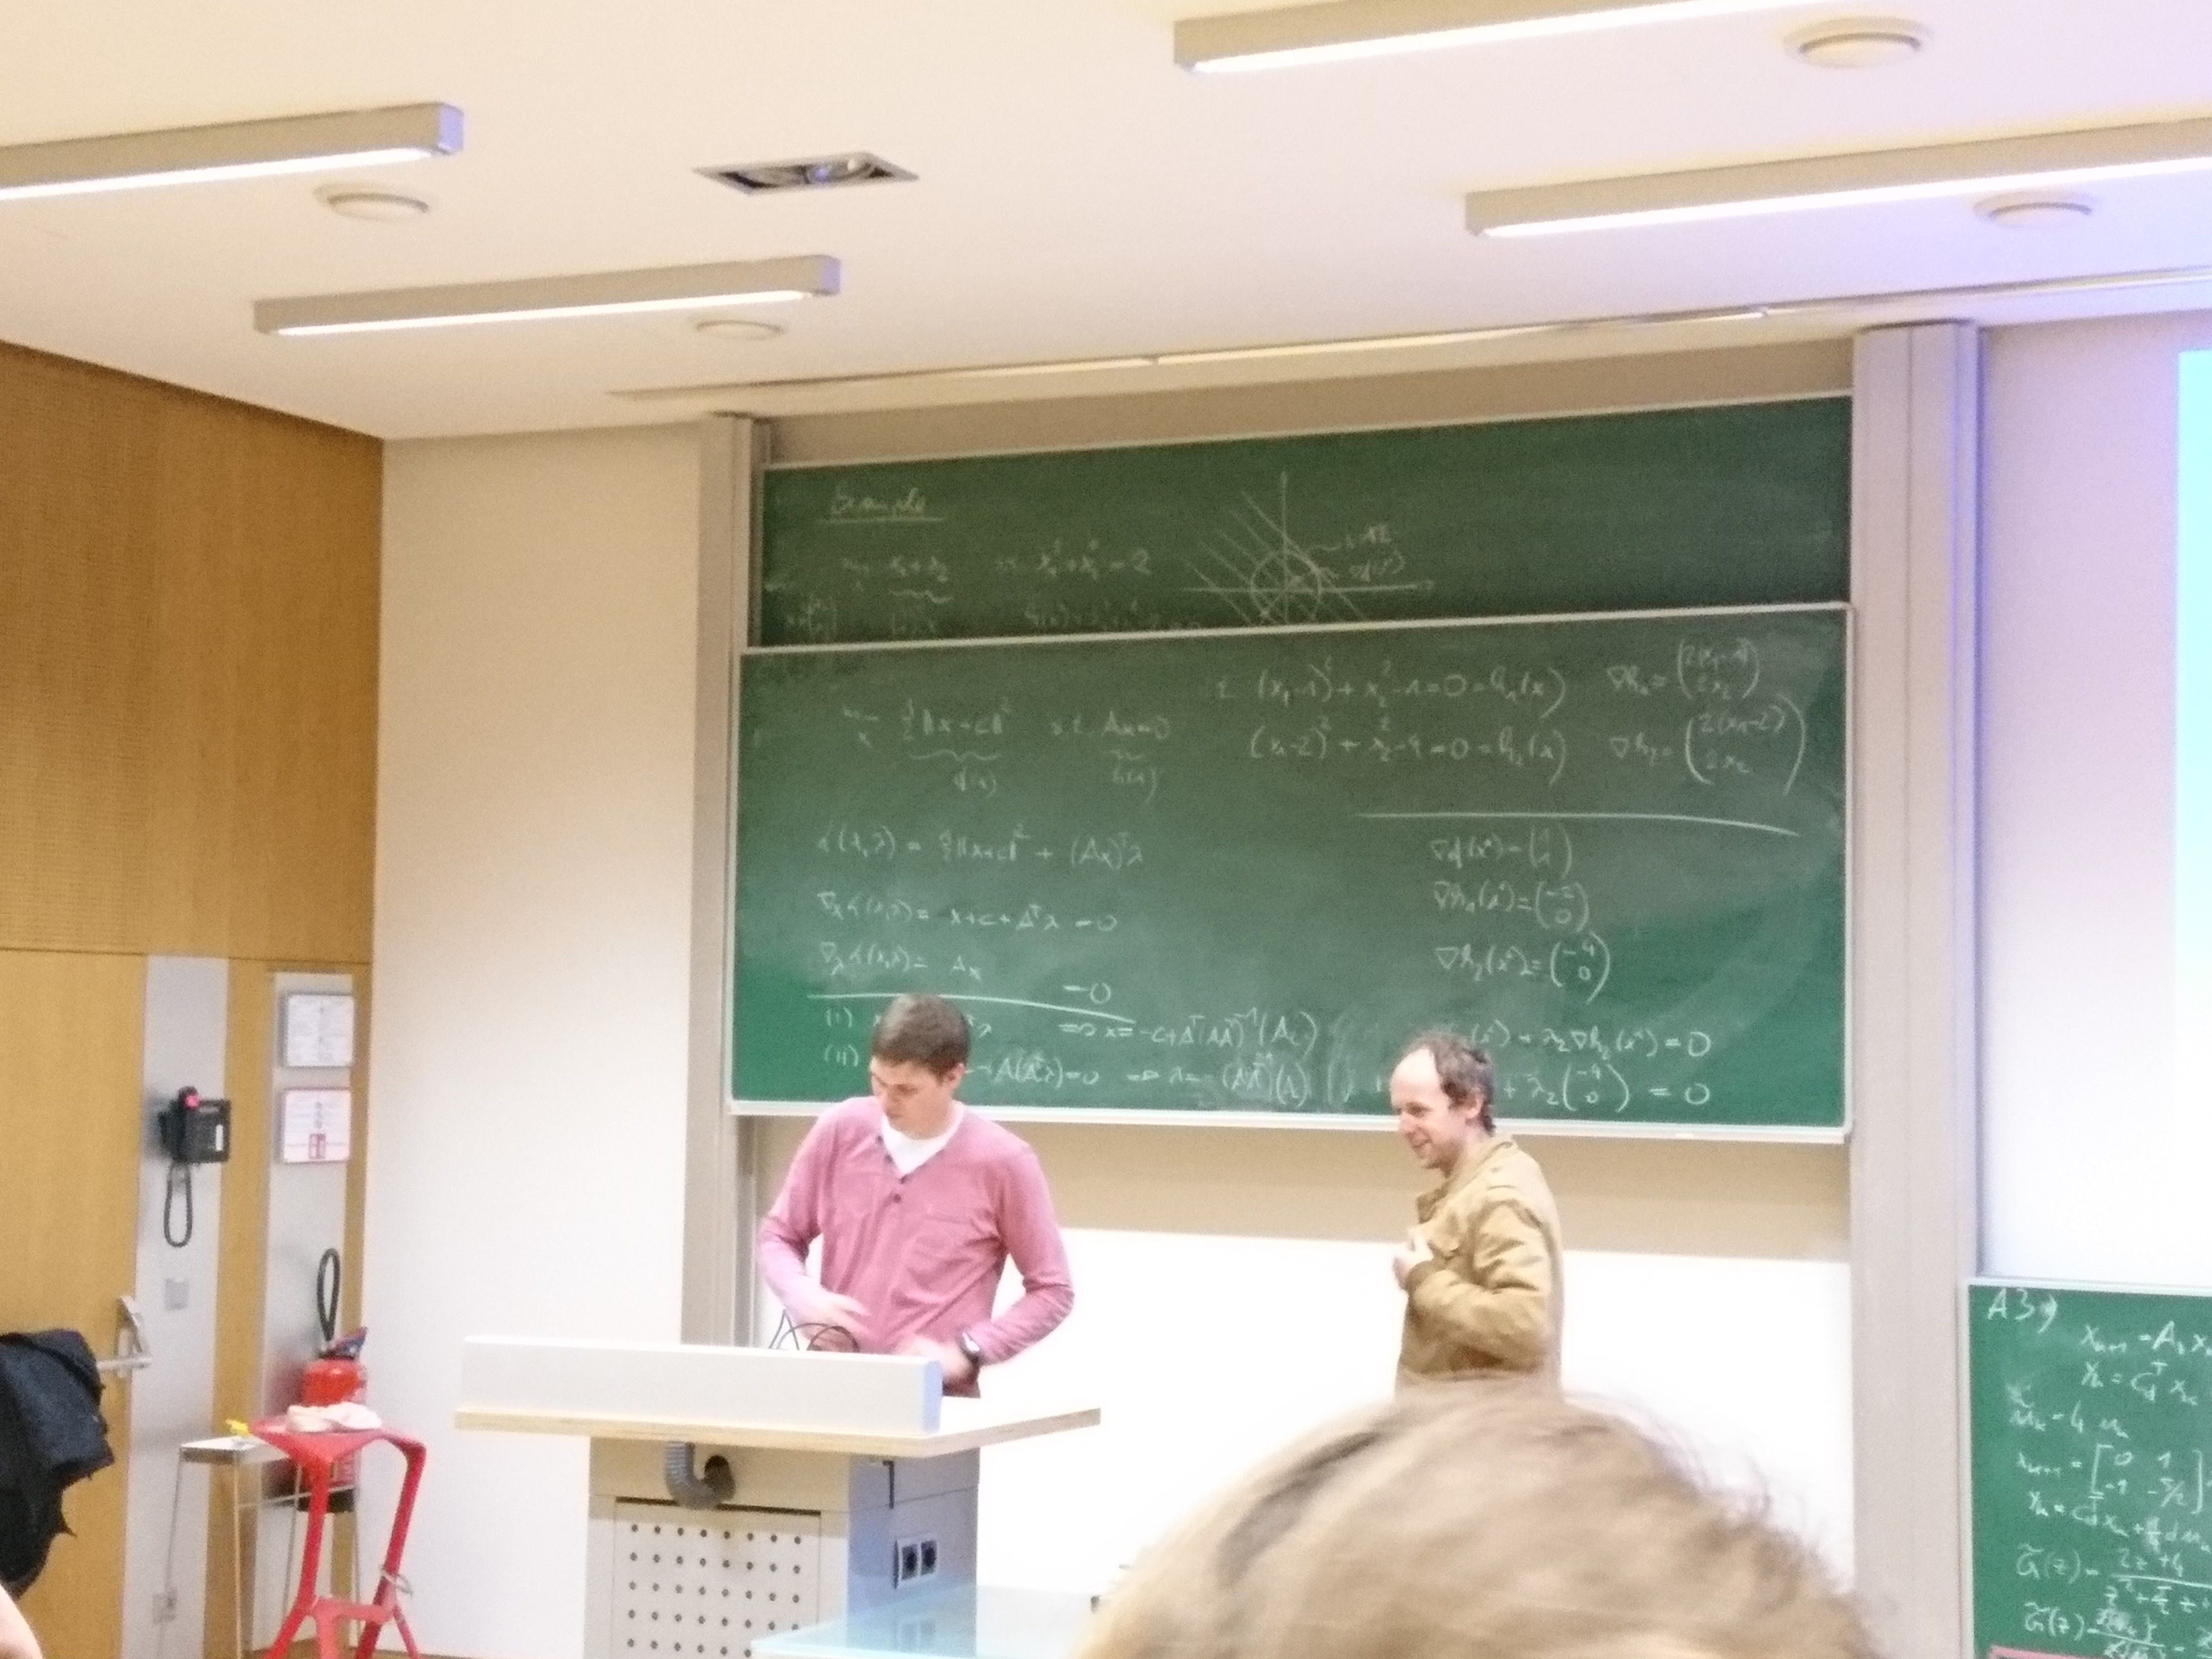
\includegraphics[width=\textwidth]{2017_01_24-ex2.jpg}
  \caption{Example 2,  24.01.2017\label{fig:ex2}}
\end{figure}
\end{document}
